\clearpage
\section{Граф вычислений}
\subsection{Абстрактная модель}
\label{sec:abstractmodel}
\begin{figure}[ht]
    \centering
    \includegraphics[width=0.8\linewidth]{graph.png}
    \caption{Структура графа}
    \label{fig:graphstructure}
\end{figure}
Граф представляет собой абстракцию, содержащую хранилище вершин графа с которыми работает пользователь в данный момент (Sync Nodes), сохраненные в графе вершины (Owning Nodes) и множество рёбер (Topology).
\begin{itemize}
    \item \textbf{Sync Nodes} -- множество вершин, объекты которых находятся у пользователя, и с которыми пользователь может работать (изменять, добавлять ассоциирующиеся с ними ребра в граф и т.п.).
    \item \textbf{Owning Nodes} -- множество вершин, сохраненных в графе, доступ к которым пользователь не имеет (заполняется при уничтожении вершины, ассоциируемой с графом, или после явного сохранения вершины пользователем).
    \item \textbf{Topology} -- множество рёбер графа.
\end{itemize}
В данный момент фреймворк позволяет пользователю создать вершины следующих типов:
\begin{itemize}
	\item \textbf{Node} -- вершина, содержащая в себе функцию от результатов входящих в неё вершин.
	\item \textbf{InputNode} -- вершина, позволяющая вносить данные в граф из различных хранилищ данных. Также может служить для хранения параметра графа вычислений, изменяющегося во время процесса оптимизации. 
\end{itemize}
\subsection{Описание алгоритма обхода графа}
\label{sec:algtraverse}
\textbf{Постановка задачи}: Требуется выделить последовательность множеств вершин (назовем их кластерами), работа с которыми может проводиться независимо внутри множеств. Кроме того вершинам $i$-го кластера требуются данные только от вершин из предыдущих кластеров. Подобное разбиение позволит с легкостью записать граф в виде обычной программы на некотором языке программирования, а так же выполнить часть операций параллельно, эффективно задействуя многоядерные системы.
\par
Последовательность кластеров должна обладать следующим свойством: Пусть $(x_1, x_2)$ - произвольное ориентированное ребро в графе. Пусть вершина $x_i$ содержится в кластере с номером $C_i$. Тогда $C_1 < C_2$. Это свойство означает: если кластеры обрабатываются последовательно, начиная с нулевого, то для любой вершины будет верно, что при старте её обработки будут обработаны все входящие в неё вершины, а значит программа сможет работать с их результатами внутри текущей вершины. Для выполнения такого разбиения разработан специальный алгоритм. 
\par
\textbf{Замечание}: Сначала будет дано описание алгоритма для графа без ориентированных циклов, а затем будут даны замечания о работе алгоритма в обходе графов, нарушающих это правило.
\begin{itemize}
	\item \textbf{Входные данные}: Множество вершин графа, разделенное на вектора вершин соответствующих типов, с указанием количества входящих в каждую вершину ребер и множество рёбер графа.
	\item \textbf{Выходные данные}: Последовательность кластеров вершин, обладаюшая вышеописанными свойствами. 
	\item \textbf{Алгоритм}: \begin{enumerate}
	    \item В множество вершин нулевого кластера заносятся все входные вершины графа. Их кластер назначается текущим.
	    \item Пока из вершин текущего кластера есть выходящие ребра, повторяем:
	    \begin{enumerate}
		\item Создаём новый пустой кластер.
	        \item Проходим по всем ребрам, выходящим из вершин текущего кластера и инкрементируем счетчик вхождений в иные вершины. Если счётчик числа вхождений в вершину достигает числа входящих в вершину рёбер - вершина добавляется в новый кластер.
		\item Назначаем новый кластер текущим и добавляем в последовательность. 
	    \end{enumerate}
	\end{enumerate}
\end{itemize}
\subsection{Доказательство корректности}
\label{sec:validalg}
Докажем корректность алгоритма методом математической индукции при условиях, описанных выше. 
\begin{itemize}
	\item \textbf{База индукции}: На нулевом шаге формируем нулевой кластер из всех входных вершин. Этот кластер сформирован корректно, т.к. между входными вершинами в графе нельзя строить ориентированные пути и предыдущих кластеров нет.
	\item \textbf{Шаг индукции}: Пусть на $i$-ом шаге корректно сформирован $i$-ый кластер. Начнем формировать $(i+1)$-ый кластер. Обозначим некоторое множество вершин графа, удовлетворяющее условию: "В вершины из множества входят лишь рёбра из вершин кластеров с индексами $0, \ldots, i$". Такое множество вершин всегда возможно составить, т.к. в постановке задачи введены необходимые условия и в Лемме \ref{lemma1} доказано, что их достаточно для упреждения такой ситуации. При составлении нового кластера из множества таких вершин он будет корректен по условию, налагаемому на рёбра. Значит его составление и добавление в последовательность означает корректность $i+1$-ого шага алгоритма.
\end{itemize}
\begin{lemma}\label{lemma1}
Если при составлении $(i+1)$-ого кластера множество вершин, удовлетворяющих условию: "В вершины из множества входят лишь рёбра из вершин кластеров с индексами $0, \ldots, i$" пустое, но при этом граф имеет не пройденные вершины, значит граф имеет ориентированный цикл.
\end{lemma}
\begin{proof}
Рассмотрим ситуации, когда вершину нельзя добавить к составляемому множеству. Можно было бы допустить, что в вершину не входит ни одно ребро. Но такие вершины должны находиться в нулевом кластере. Тогда остается единственный вариант: в любую вершину из множества непройденных входит хотя бы одно ребро из другой непройденной вершины. Тогда на непройденных вершинах можно построить ориентированный цикл.
\end{proof}
\textbf{Замечание}: Данный алгоритм также позволяет проверить граф на ацикличность и на достижимость произвольной вершины из вершин нулевого кластера. \newline
\textbf{Решение}: Во время обхода графа считать число вершин, добавленных в кластеры и сравнивать его с полным числом вершин. Ориентированные циклы могут состоять только из вершин, которые могут иметь входящие и исходящие рёбра. При встрече алгоритма с вершиной ориентированного цикла он не сможет перейти в неё, т.к. существует ребро, являющееся частью этого цикла, но ещё не пройденное алгоритмом, ведь оно исходит из вершины, прежде которой надо посетить ту, в которую алгоритм пытается посетить в данный момент. Следовательно эта вершина не будет добавлена ни в один из кластеров.
\subsection{Программное представление вершин}
\label{sec:softwarepresentationnodes}
\begin{figure}[ht]
    \centering
    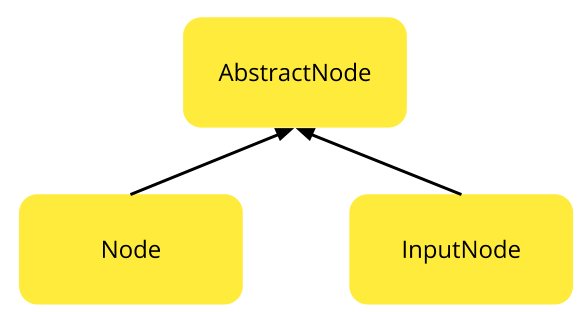
\includegraphics[width=0.8\linewidth]{node_hierarchy.png}
    \caption{Иерархия классов вершин}
    \label{fig:nodes_hierarchy}
\end{figure}
Все типы вершин представлены иерархией классов, отображенной на рисунке \ref{fig:nodes_hierarchy}
\begin{itemize}
    \item \textbf{AbstractNode} -- абстрактный класс, инкапсулирующий общие для всех вершин поля: имя, число входящих рёбер, тензор результата.
    \item \textbf{Node} -- класс, позволяющий хранить объект операции (operation).
    \item \textbf{InputNode} -- класс, позволяющий хранить объект-загрузчик (loader), необходимый для загрузки данных в граф из сторонних источников.
\end{itemize}
\subsection{Программное представление графа}
\label{sec:softwarepresentationgraph}
Граф представлен классом Graph в пространстве имен athena::core. Основные его поля выполнены следующим образом:
\begin{itemize}
    \item \textbf{Sync Nodes} -- представляет собой объект std::unordered\_set, содержащий id вершин, принадлежащих графу, но объекты которых находятся не в хранилище Owning Nodes.
    \item \textbf{Owning Nodes} -- представляет собой кортеж векторов, позволяющий содержать объекты всех существующих типов вершин.
    \item \textbf{Topology} -- множество рёбер графа, представленное с помощью std::vector.
\end{itemize}
\subsection{Программное представление алгоритма обхода графа}
\label{sec:softwarepresentationgraph}
Пусть имеется $k$ входных вершин графа, $n$ вершин в графе всего, $m$ рёбер в графе всего.
\textbf{Входные данные}: Кортеж векторов вершин графа, с указанием количества входящих в каждую вершину ребер и множество рёбер графа, представленное неотсортированным вектором.
\par
\textbf{Выходные данные}: Вектор кластеров вершин.
\par
\textbf{Алгоритм}: \begin{enumerate}
    \item Отсортировать вектор рёбер. Назначить каждой вершине индекс, показывающий начало подвектора исходящих из неё рёбер. Используется сортировка IntroSort - Сложность $O(m*log(m))$
    \item В вектор вершин нулевого кластера заносятся все входные вершины графа. Их кластер назначается текущим. - Сложность $O(k)$
    \item Пока из вершин текущего кластера есть выходящие ребра, повторяем:
    \begin{enumerate}
        \item Проходим по всем ребрам, выходящим из вершин текущего кластера и инкрементируем счетчик вхождений в иные вершины. - Суммарныая сложность $O(m)$
        \item Все иные вершины, счетчик соответствующий которым сравнялся с числом входящих в них на данной итерации рёбер кладем в новый кластер, назначаем его текущим и добавляем в последовательность. - Суммарная сложность $O(n-k)$
    \end{enumerate}
\end{enumerate}
\par
\textbf{Сложность алгоритма}: $O(m*log(m)) + O(m) + O(n-k) + O(k) = O(m*log(m))$
